\section{Implementation}
\label{sec:impl}

In this section, the implementations of the \textit{rf95modem} firmware, the device-to-device messaging application, and the integration into disruption-tolerant networking software are presented.

\subsection{Modem Firmware}

\begin{figure}[ht!]
    \centering
    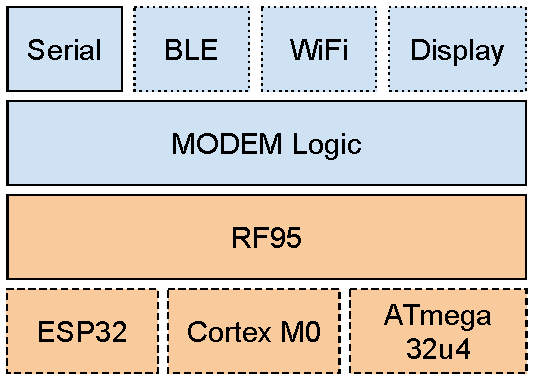
\includegraphics[width=.5\columnwidth]{gfx/rf95modem-arch.pdf}
    \caption{Overview of the \textit{rf95modem} architecture.}
    \label{fig:rf95modem_arch}
\end{figure}

Since a \textit{rf95modem} should be controlled by AT commands over all of its available connection mechanisms, handling such commands is an essential part of the implementation. 
Therefore, this functionality is shared across all supported hardware platforms and connection mechanisms, as shown in Figure~\ref{fig:rf95modem_arch}. 
Here, the software components are displayed in blue while the rest represents the underlying hardware modules.
For interaction with users and software, the serial device interface, usually accessible via USB, is always active. 
Furthermore, the in-/output functions may also be hooked to the Bluetooth Low Energy or WiFi modules we developed, if enabled at compile time. 
Any output is mirrored to all enabled interfaces that can be used simultaneously. 

To achieve optimal results on various  hardware platforms and configurations, all features and hardware configurations can be set using build flags.
For example, the SPI pin configuration and the underlying CPU architecture must be configured, as well as the base LoRa frequency. 
Currently, we support ESP32-based boards with RF95-compatible LoRa transceivers as well as some Cortex M0 and ATmega32u4-based boards, such as the ones produced by Adafruit for the Feather line of devices.

For the ESP32 boards, we provide a WiFi mode featuring two different ways of communication that can be used in parallel. 
In both cases, an access point is opened by the device itself for modem users to connect to.
The first mode is UDP-based and just broadcasts the modem output to the local network and interprets incoming AT commands via datagram packets. 
This is especially useful if many local devices want to listen on incoming transmissions. 
The second mode is the TCP exclusive mode. 
Here, a single TCP connection is accepted that can then control the model similarly to a serial interface. 
Since the ESP32 boards also feature Bluetooth, they can be used to announce a BLE characteristic for interaction with the \textit{rf95modem}. 
This interface acts similarly to the others by interpreting strings received via a write characteristic as AT modem commands. 
The output is shared via a notify characteristic to which devices can subscribe. 
BLE is supposed to have a payload limit of 20 bytes, and thus splitting the serial output into smaller chunks is necessary. 
Our tests on various platforms, e.g., iPhones and Raspberry Pis, have shown that sending much larger packets via BLE is often also possible and much more efficient. 
Therefore, sending overlong frames via BLE can optionally be activated during runtime via a specific AT command.
Finally, there is also a software module to support OLED displays as they are pretty common on TTGOs and Heltecs ESP32 devices. 
If enabled at compile time, these can be used to display status information such as the current frequency, packets received, and number of packets transmitted, which can be used for debugging or providing statistical information at a glance without the need for special hardware or software.

Since all board-specific features can be configured at compile time, the firmware can be custom-tailored to fit even very resource-limited devices. 
Enabling all features at once results in a large firmware, which requires more flash memory and a custom partition layout, but still works on the most common ESP32 boards. 
Due to the fact that all output is mirrored between the interfaces, one can easily use two interfaces in parallel, e.g., debugging the BLE communication via an attached serial cable.
The firmware is completely written in C/C++ using the Arduino SDK and PlatformIO as a build system.
% To make the features of \textit{rf95modem} easily accessible to various applications, we also provide language bindings for the serial interface to Rust\footnote{\url{https://github.com/gh0st42/rf95modem-rs}} and Go\footnote{\url{https://github.com/dtn7/rf95modem-go}}.

\begin{figure}
\centering
\begin{subfigure}{.5\textwidth}
  \centering
  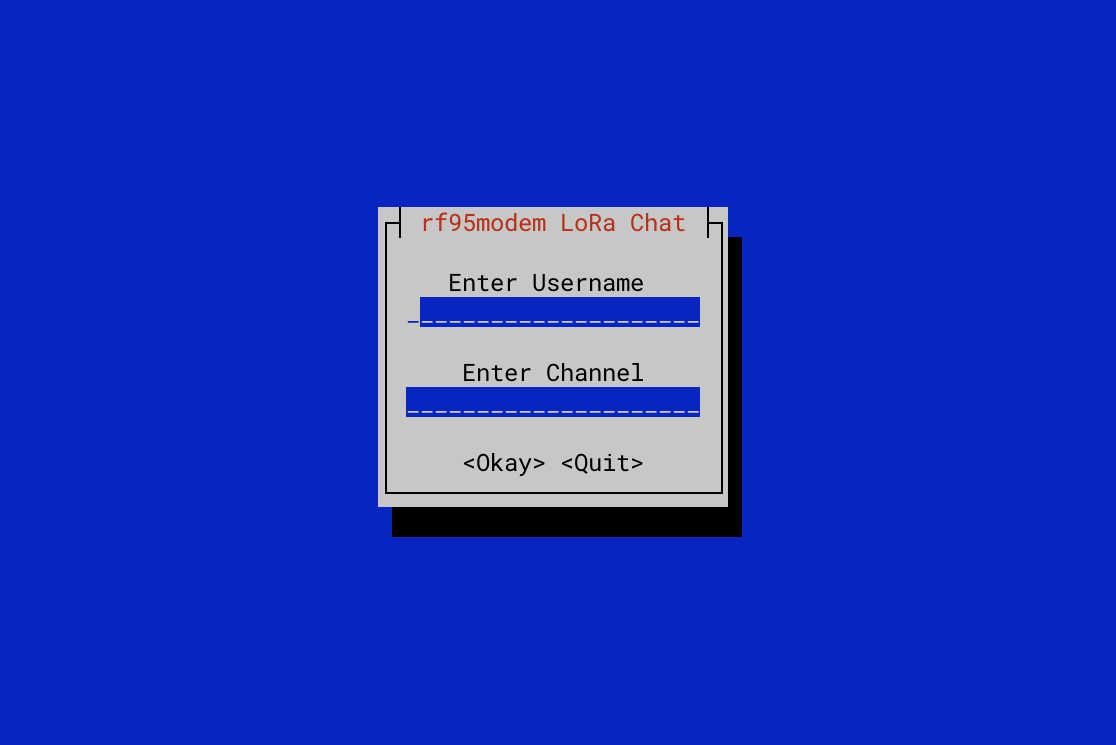
\includegraphics[width=.95\linewidth]{gfx/lorachat_1.png}
  \caption{Login screen}
  \label{fig:lorachat:login}
\end{subfigure}%
\begin{subfigure}{.5\textwidth}
  \centering
  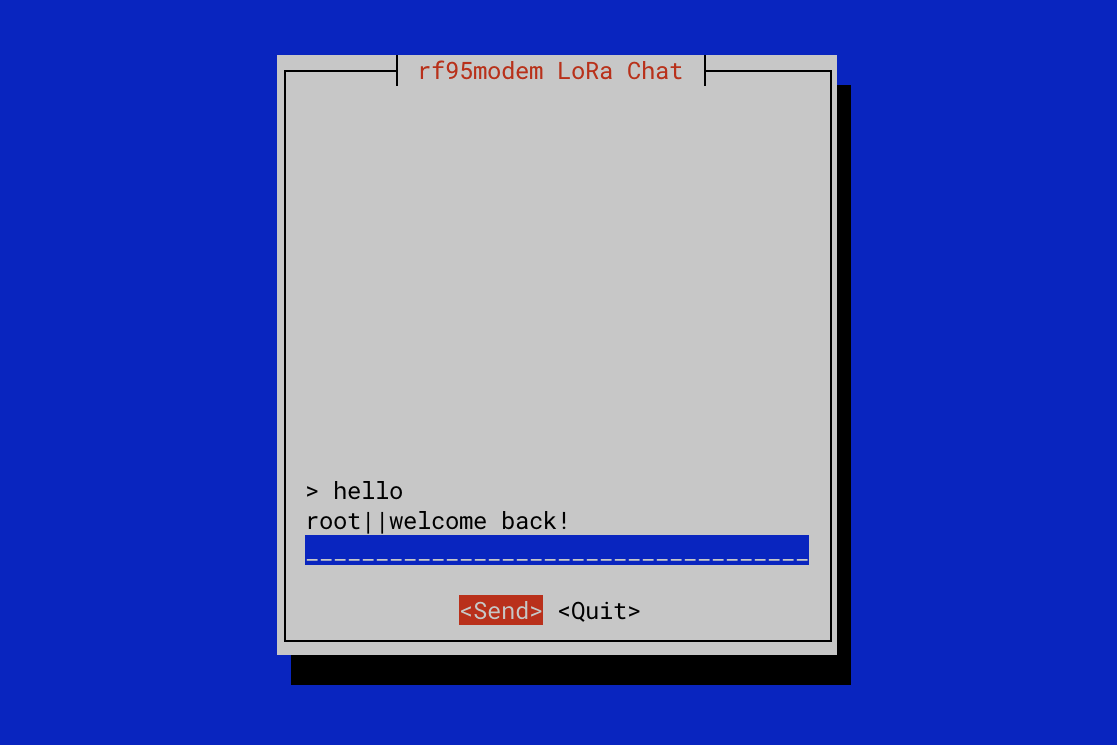
\includegraphics[width=.95\linewidth]{gfx/lorachat_2.png}
  \caption{Chat interface}
  \label{fig:lorachat:chat}
\end{subfigure}
\caption{Console-based \textit{rf95modem} LoRa chat example.}
\label{fig:lorachat}
\end{figure}


\subsection{A Device-To-Device Messaging Application}
To satisfy the requirements of the messaging application, we provide two different approaches.
First, we provide a console-based user interface for traditional computers, as shown in Figure~\ref{fig:lorachat}\footnote{\url{https://github.com/gh0st42/rf95modem-rs}}.
Second, for the mobile version of the application (BlueRa), we used the Flutter UI toolkit\footnote{\url{https://flutter.dev}}.
Flutter allows developers to create platform independent apps for both major mobile operating systems, iOS and Android, using the same code base.

\begin{figure}[ht!]
    \centering
    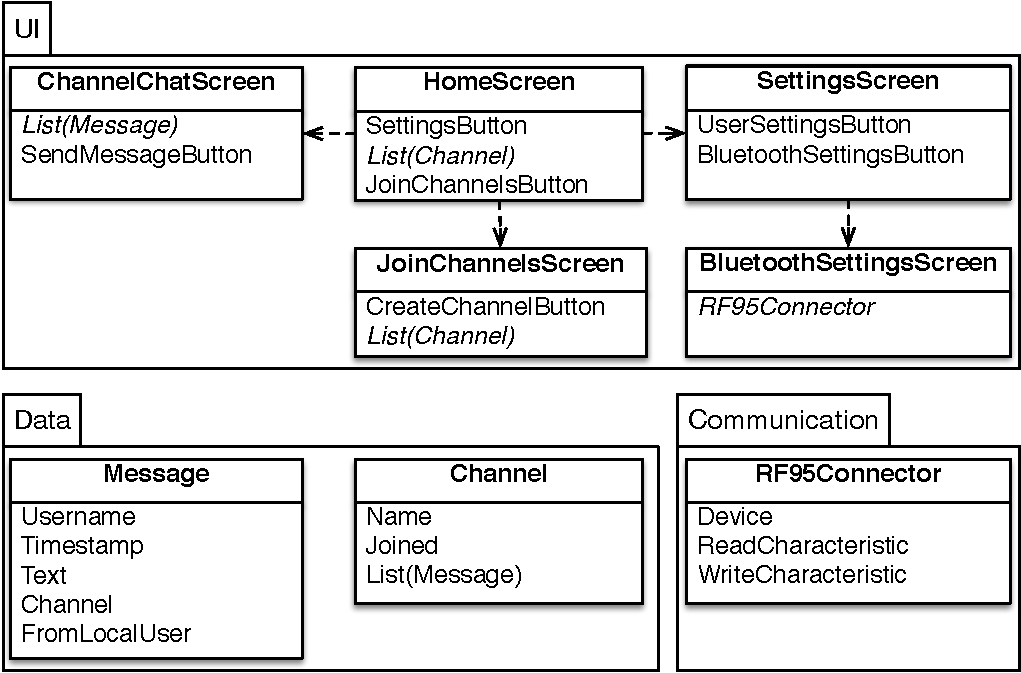
\includegraphics[width=.7\columnwidth]{gfx/bluera-uml.pdf}
    \caption{Overview of the components of the app.}
    \label{fig:app_uml}
\end{figure}

Figure~\ref{fig:app_uml} gives a simplified overview of the components of the app.
The top block shows the UI classes.
The application starts at the home screen, which contains a path to the settings, a list view of the available channels and a path for joining to new channels or to create channels.
On the left, users can change their usernames or manage the app's Bluetooth connection, each in their own screens (the username settings screen is not shown in the figure).
When the app's route heads over to the \emph{JoinChannelScreen}, a list of available channels that the user has not joined yet is presented.
Additionally, this screen enables the user to create new channels.
The final screen is the chat screen itself, where the user can see a history of the messages in this particular channel as well as a text field for creating and sending new messages.

\begin{figure}[ht!]
    \centering
    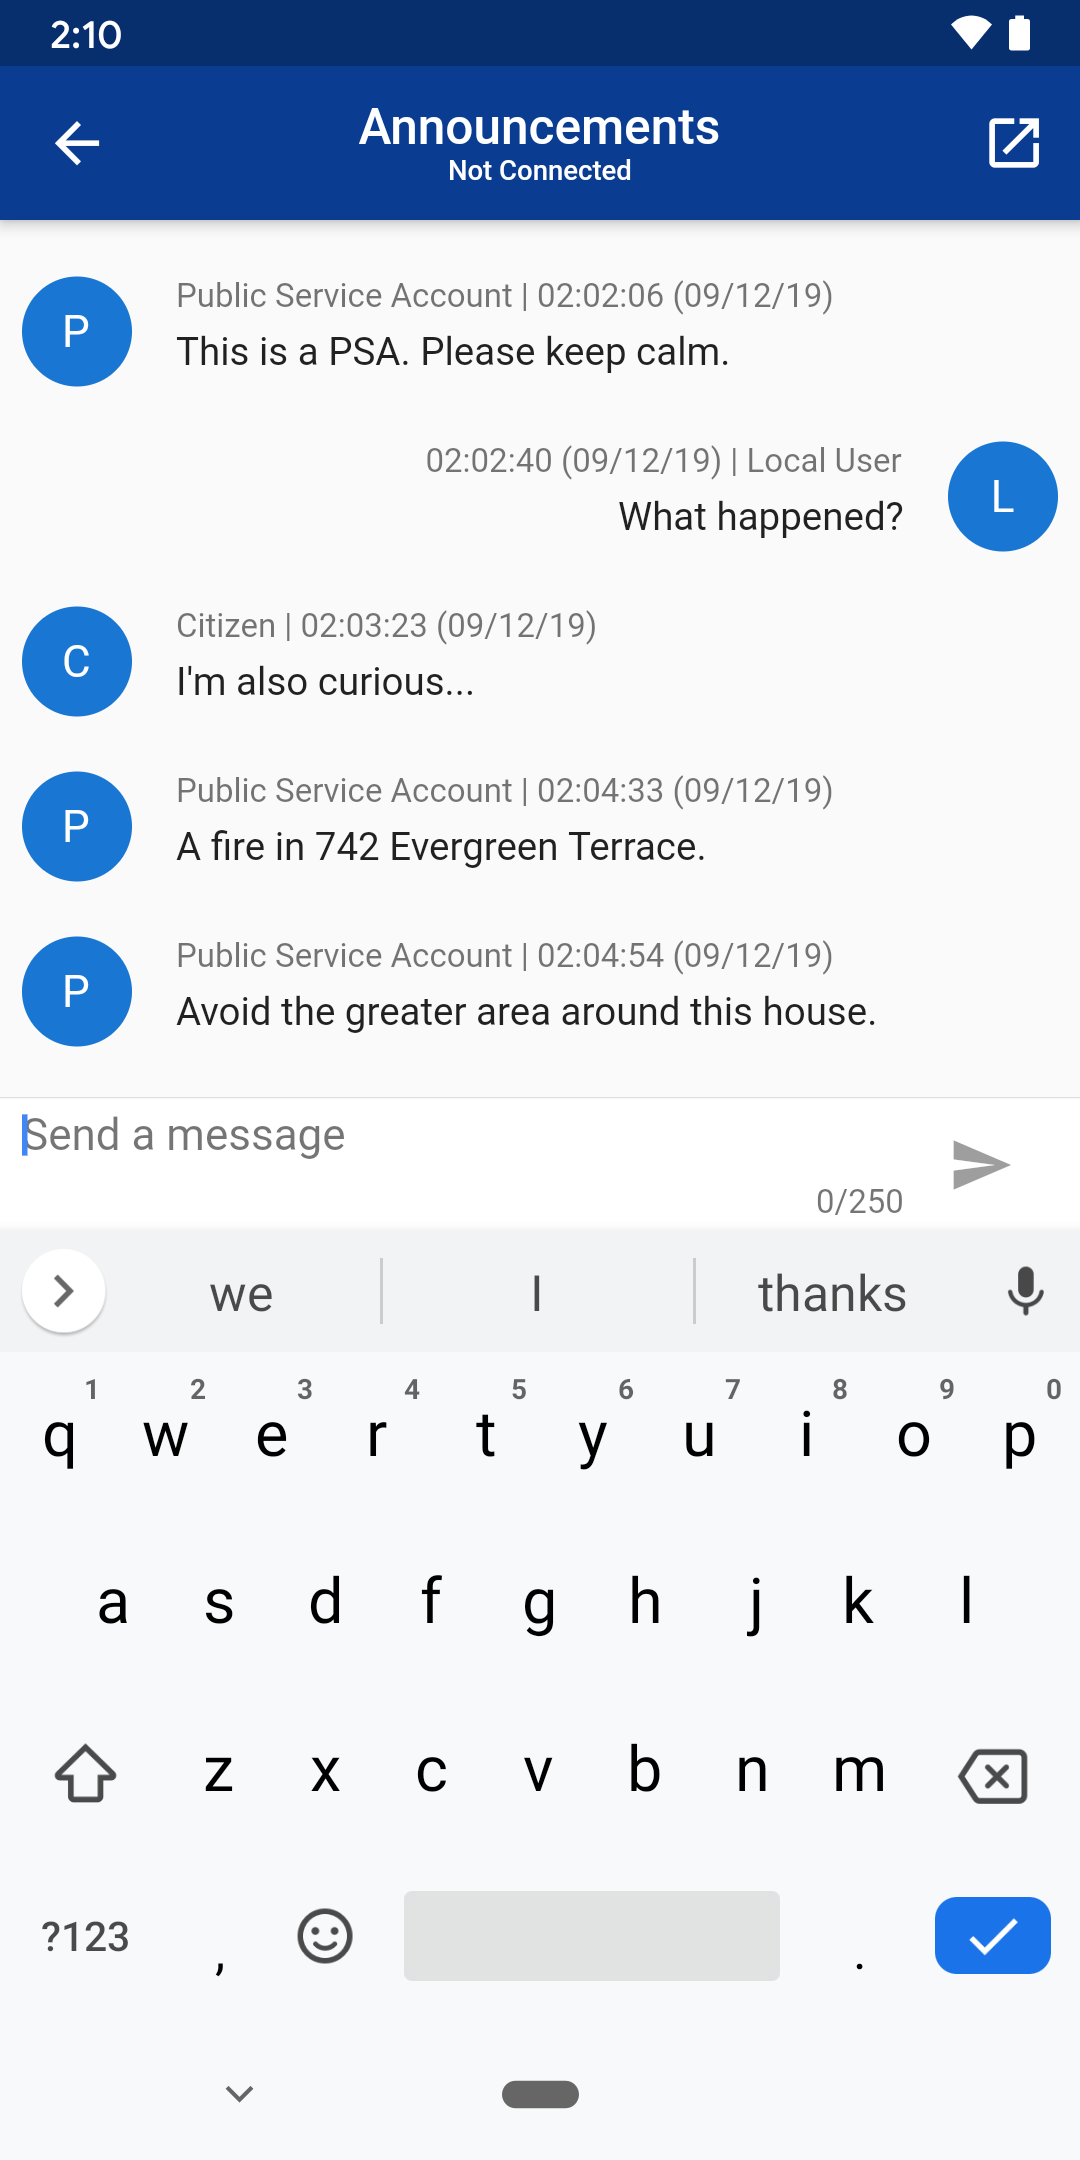
\includegraphics[width=0.4\textwidth]{gfx/bluera-screenshot.png}
    \caption{Screenshot of the chat screen for the announcements channel.}
    \label{fig:app_screenshot}
\end{figure}

Figure~\ref{fig:app_screenshot} shows the chat screen for the announcements channel.
Using this common chat UI/UX, the user gets a familiar look and can start messaging immediately, without the need of getting familiar with a special UI.

As indicated by the \emph{Channel} module in Figure~\ref{fig:app_uml}, a channel has a name, an indicator whether the local user has joined this channel and a list of messages.
A message, on the other hand, contains the name of the user who sent this message, a timestamp, the text itself, the channel name and an indicator whether the message was sent from the local user.

The connection to the \textit{rf95modem} device is implemented in its own module, \emph{RF95Connector}.
This module holds the device ID and Bluetooth connection state, as well as the read and write characteristics for the serial communication service.
Additionally, this module also implements data and message handling.
When sending a new message, all required data is serialized to the appropriate format and sent to the modem using the write characteristic.
Furthermore, a receive listener gets notified, as soon as new data is available in the read characteristic.
The received data is parsed and the internal channel- and message database is updated.
If the channel of the received message is already present, the message is appended to the channel's message list.
Otherwise, a new channel in the local database is created with the received message.
This new channel will be presented in the \emph{JoinChannelScreen}, so that users can join this channel if they want to.

We used a simple communication protocol for sending and receiving messages.
It consists of the channel name, a user name, an optional location and the actual message separated by vertical bars.
Following this simple protocol design, it is possible for any communication device to communicate with the app, regardless of the capabilities and available serialization libraries like JSON, CBOR, or Protocol Buffers.


\subsection{Disruption-tolerant Networking}
To use LoRa in disruption-tolerant networking, we have extended the DTN7 implementation\footnote{\url{https://github.com/dtn7/dtn7-go}} introduced by \cite{penning2019dtn7}.
Within the DTN context, the communication interface for bundle exchange between nodes is called convergence layer.
We have implemented the convergence layer interface provided by DTN7 to achieve LoRa support.

To integrate \textit{rf95modem}'s serial link into DTN7, we have first developed a  library\footnote{\url{https://github.com/dtn7/rf95modem-go}},  written in the Go programming language.
This library's main task is to provide Golang typical interfaces for writing and reading data streams through \textit{rf95modem}.
Furthermore, status information of the modem can be read and reconfigured.

% generated with UMLet, source file is dtn7-bbc.uxf
\begin{figure}[ht!]
    \centering
    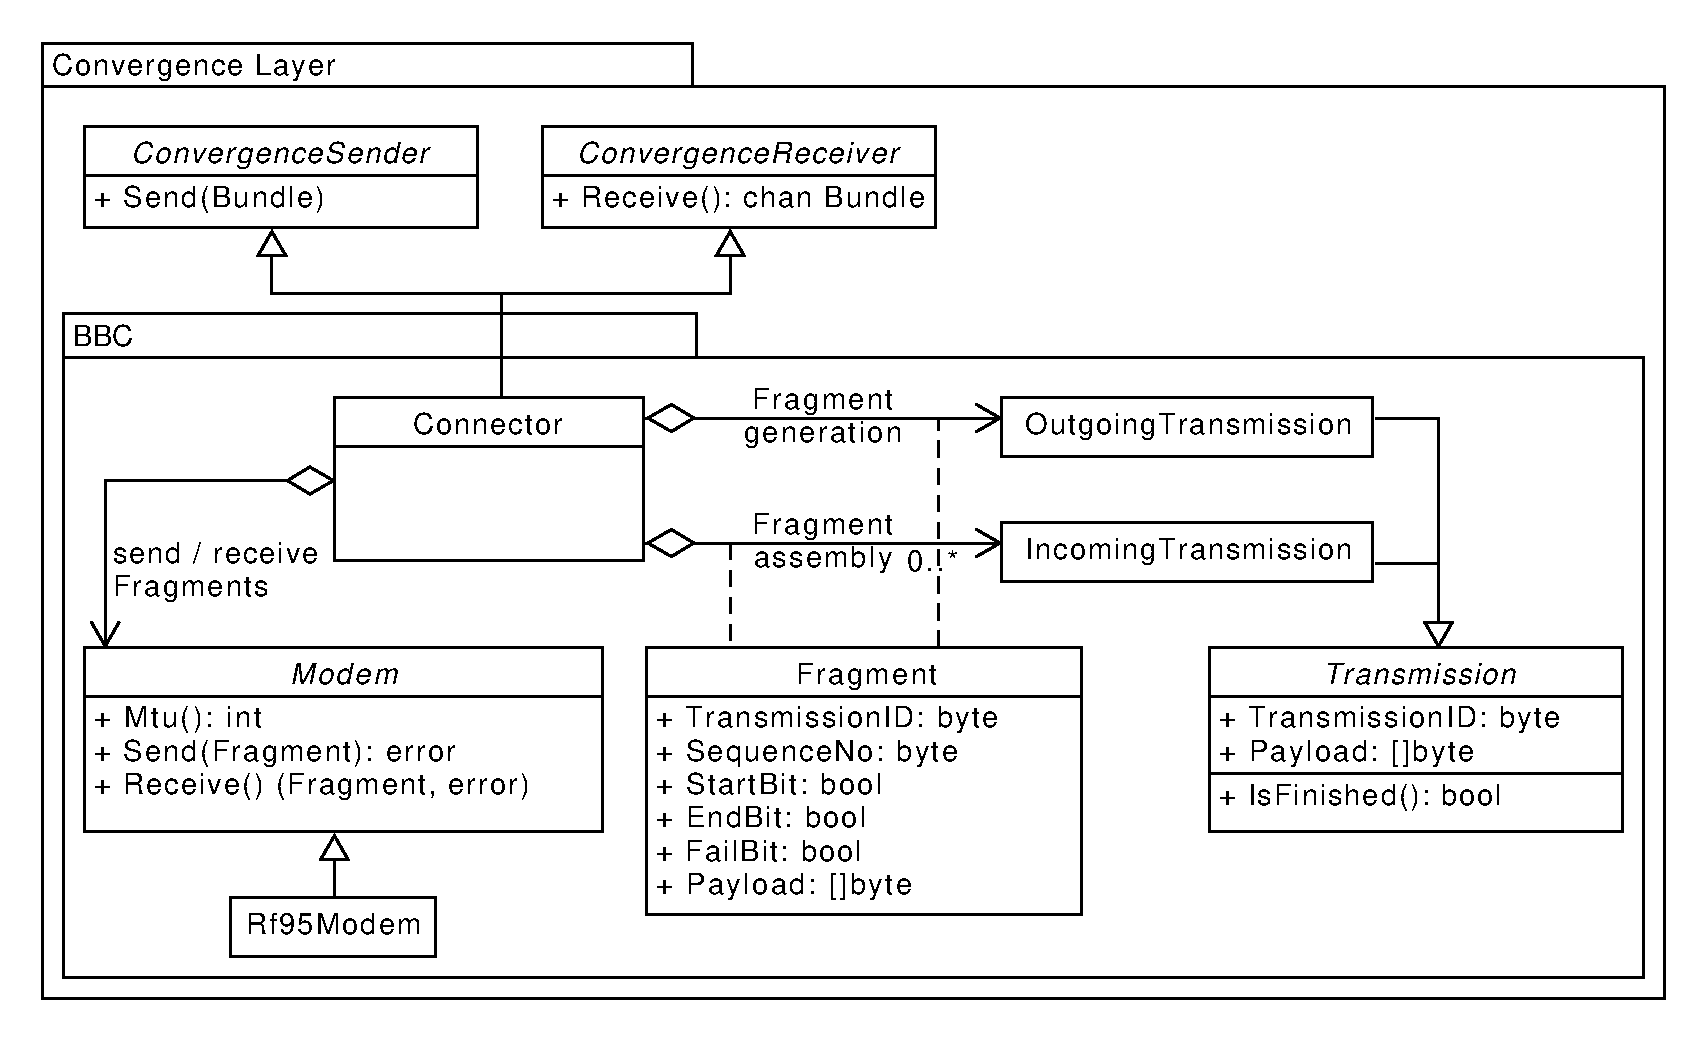
\includegraphics[width=1.0\columnwidth]{gfx/dtn7-bbc.pdf}
    \caption{Simplified implementation model of the Bundle Broadcasting Connector.}
    \label{fig:dtn7_bbc_uml}
\end{figure}

Until now, DTN7 only had support for unicast convergence layers, while the transmission of LoRa packets corresponds to a broadcast.
Since most broadcast technologies are similar in structure, we first developed a generic broadcasting convergence layer, the Bundle Broadcasting Connector (BBC).
Its simplified implementation model is shown in Figure~\ref{fig:dtn7_bbc_uml}.

The main component of the BBC package is the connector that implements DTN7's convergence layer interfaces for both sending and receiving bundles.
The connector itself communicates with a modem, which is an interface implemented in \textit{rf95modem-go} and a mock object for testing.
Each modem reports its MTU such that transmissions can be fragmented accordingly.

With regard to transmissions, the BBC makes a distinction between incoming and outgoing ones.
Both types have an identifier and can determine whether they have finished.
If a bundle should be sent via our BBC, an outgoing transmission with a new identifier will be generated.
This identifier is derived from the node.
Every node is initialized with a random identifier, which is then incremented for each transmission.
The payload is the \texttt{xz}\footnote{\url{https://tukaani.org/xz/format.html}} compressed bundle.
As long as the transfer is not completed, the connector requests a new fragment.
Its length including headers must not exceed the modem's MTU.
This is then handed to the modem, which broadcasts it via LoRa in our case.
 
\begin{figure}[ht!]
    \centering
    
    \begin{bytefield}[bitformatting={\small\bfseries},bitwidth=0.05\linewidth]{8}
        \bitheader{0-7} \\
        
        \begin{rightwordgroup}{Header}
            \bitbox{8}{Transmission ID} \\
            \bitbox{5}{Sequence No.} & \bitbox{1}{Start} & \bitbox{1}{End} & \bitbox{1}{Fail}
        \end{rightwordgroup} \\
        
        \bitbox[lrt]{8}{Payload} \\
        \skippedwords \\
        \bitbox[lrb]{8}{}
    \end{bytefield}
    
    \caption{Protocol specification of a fragment.}
    \label{fig:fragment_protocol}
\end{figure}

The network protocol specification of a fragment is shown in Figure~\ref{fig:fragment_protocol}.
A fragment itself consist of a header of two bytes, followed by the payload.
In the header, the identifier of the transmission is referenced next to a sequence number.
Each fragment contains the incremented sequence number of its predecessor.
Thus, lost fragments can be detected in advance.
In addition, the header has three flags.
The start bit indicates the beginning of a new transmission, while the end bit indicates its end.
A fail bit is set for status packets that imply the absence of fragments.

When receiving fragments, the modem forwards them to the connector.
This checks whether the transmission identifier is already known.
If this is the case, the fragment is added to the incoming transmission.
Otherwise, a new incoming transmission is created.
Once the transmission is finished, the entire payload is extracted and decompressed.
The resulting bundle will be passed back to DTN7's logic.
However, if a reception error occurred, e.g., due to a skipped sequence number, a status packet is sent.
This packet is equal to the last fragment, except that the fail bit is set and the payload is empty.
Reception of such a packet by the sender marks the transmission as faulty.
As a result, DTN7 will re-trigger the transmission at a later time.
